% Copyright 2026 Sreeram Anil
% SPDX-License-Identifier: CC-BY-4.0
% =============================================================================
%  Cooperative interval observer
% =============================================================================
\chapter{Cooperative Interval Observer (IntervalObserver)}
\label{ch:intervalobserver}

\section*{At a glance}
\begin{tabular}{@{}l>{\raggedright\arraybackslash}p{0.76\textwidth}@{}}
Family & Deterministic observers \\
Header & \texttt{include/estkit/observers/interval\_observer.hpp} \\
Registered name & \texttt{IntervalObserver} \\
State dimension & $2n_x = 8$ (lower and upper trajectories) $+\,n_x$ for the embedded point estimator \\
Cost per step & $\mathcal{O}(n_x n_u)$ plus $n_{\mathrm{samp}}$ Jacobian evaluations; $\approx 0.8\,\mu$s/step measured \\
Primary references & \cite{gouze2000interval,raissi2012interval,mazenc2011interval,efimov2016interval,smith1995monotone} \\
Interval capability & yes --- reports $[\soc_{\mathrm{lo}},\soc_{\mathrm{hi}}]$ through \texttt{with\_bounds} \\
\end{tabular}

\section{Motivation and aerospace/BMS relevance}
Every other estimator in this study reports a number.  A Kalman filter additionally reports a
covariance, but that covariance is the covariance of the \emph{assumed} model, and in exactly the
scenarios where it matters --- a biased sensor, a faded cell, a wrong resistance --- the assumption
is false and the $\pm2\sigma$ band is a fiction.  An interval observer reports two numbers with a
different status: under stated bounds on the uncertainties, the truth is \emph{guaranteed} to lie
between them.

For an aircraft this is the quantity the regulation actually wants.  A reserve-energy declaration
is a worst-case statement, and a set-membership bound is a worst-case statement; a standard
deviation is not.  Gouz\'e, Rapaport and Hadj-Sadok \cite{gouze2000interval} introduced interval
observers for uncertain biological systems, Ra\"issi, Efimov and Zolghadri
\cite{raissi2012interval} extended them to a broad class of nonlinear systems, and Mazenc and
Bernard \cite{mazenc2011interval} and Efimov and Ra\"issi \cite{efimov2016interval} developed the
design theory.  The structural requirement is \emph{cooperativity} (monotonicity) of the error
dynamics \cite{smith1995monotone}, and this chapter is largely about what that requirement costs
on a battery.

\section{Problem statement and assumptions}
No probabilistic assumption.  Every uncertainty is bounded:
\begin{align}
|v_k| &\le \bar{v} && \text{measurement error (noise, quantisation, outliers)} , \label{eq:io-vbar}\\
|\delta u_{j,k}| &\le \bar{u}_j && \text{error of input channel } j , \label{eq:io-ubar}\\
|w_{i,k}| &\le \bar{w}_i && \text{per-step model error on state } i . \label{eq:io-wbar}
\end{align}
\begin{assumption}[Initial enclosure]\label{as:io-init}
$\vx_{\mathrm{lo},0}\le\vx_0\le\vx_{\mathrm{hi},0}$ componentwise.
\end{assumption}
\begin{assumption}[Cooperativity]\label{as:io-coop}
$\mA = \partial f/\partial\vx\ \ge 0$ elementwise (the discrete analogue of a Metzler matrix).
\end{assumption}
The cell model satisfies \Cref{as:io-coop} by construction: $\mA = \diag(1,a_1,a_2,a_h)$ with
$a_i\in(0,1)$.  Any negative off-diagonal entry that another model might have is handled by
widening the interval with $|\mA_{ij}|(x_{\mathrm{hi},j}-x_{\mathrm{lo},j})$, at the cost of
conservatism.

\section{Derivation}

\subsection{Time update}
If $f$ is order preserving --- which \Cref{as:io-coop} guarantees --- then
$\vx_{\mathrm{lo}}\le\vx\le\vx_{\mathrm{hi}}$ implies
$f(\vx_{\mathrm{lo}},\vu)\le f(\vx,\vu)\le f(\vx_{\mathrm{hi}},\vu)$.  Adding the input and model
uncertainty gives
\begin{equation}
x^-_{\mathrm{hi},i} = f_i(\vx_{\mathrm{hi}},\vu) + \sum_j\big|B_{ij}\big|\bar{u}_j + \bar{w}_i ,
\qquad
x^-_{\mathrm{lo},i} = f_i(\vx_{\mathrm{lo}},\vu) - \sum_j\big|B_{ij}\big|\bar{u}_j - \bar{w}_i ,
\label{eq:io-pred}
\end{equation}
with $\mB = \partial f/\partial\vu$.  The input term is a first-order over-approximation; for the
cell it is exact on the SOC channel, where $f_{\soc}$ is affine in $i$ for a fixed sign of the
current, and first order elsewhere.

\subsection{Measurement update and the cooperativity condition}
Apply a correction of the same form as \eqref{eq:lue-update} to each bound.  Using the mean-value
theorem on the scalar output, $h(\vx_{\mathrm{hi}}^-,\vu)-h(\vx,\vu) = \mC(\bm{\xi})
(\vx_{\mathrm{hi}}^- - \vx)$ for some $\bm{\xi}$ on the segment, so with
$\bar{\veps} = \vx_{\mathrm{hi}} - \vx \ge \bm{0}$,
\begin{equation}
\bar{\veps}^+ = \big(\mI - \mL\mC(\bm{\xi})\big)\,\bar{\veps}^- + \mL v + \text{(inflation)} .
\label{eq:io-errup}
\end{equation}
For the upper bound to stay above the truth for \emph{every} admissible $\bar{\veps}^-\ge\bm{0}$
we need $(\mI-\mL\mC)\ge0$ elementwise, i.e.
\begin{equation}
\boxed{\quad 1 - L_i C_i \ \ge\ 0 \quad\text{and}\quad -L_i C_j \ \ge\ 0 \ \ (i\neq j)
\quad\text{for every } \mC \text{ in the hull over the box.}\quad}
\label{eq:io-coop}
\end{equation}
The $\mL v$ term is covered by adding $|\mL|\bar{v}$ to the upper bound and subtracting it from
the lower one.

\subsection{Feasibility: cooperativity forces a zero gain for the cell}
\label{sec:io-feas}
$\mC = [\partial\ocv/\partial\soc,\ -1,\ -1,\ M]$ has \emph{mixed signs}: the OCV slope and the
hysteresis coefficient are positive, the RC coefficients are negative.  Apply \eqref{eq:io-coop}
row by row.  Row $i=\soc$: $j=v_1$ and $j=v_2$ give $-L_{\soc}(-1)\ge0\Rightarrow L_{\soc}\ge0$,
while $j=h$ gives $-L_{\soc}M\ge0\Rightarrow L_{\soc}\le0$.  Hence $L_{\soc}=0$.  The same
argument applied to every row gives $\mL = \bm{0}$.  Cooperativity and output injection are
incompatible for this $\mC$, and the ``obvious'' interval observer degenerates to open-loop
bound propagation.

This is the standard obstruction in the interval-observer literature and the usual remedy is a
change of coordinates in which the error dynamics become cooperative
\cite{raissi2012interval,mazenc2011interval}.  Here a simpler and equally rigorous route is
available, because the obstruction is caused by \emph{one} column.

\subsection{Neutralising the blocking columns}
Correct a single state $j^\star$ (by default the one with the largest DC disturbance gain,
\eqref{eq:pi-Gauto}; SOC for the cell) and take the sign of $\ell = L_{j^\star}$ from
$C_{j^\star}$.  For $\ell>0$ the condition $-\ell C_j\ge0$ requires $C_j\le0$; call the columns
$j\ne j^\star$ with $C_j>0$ \emph{blocked}.  Their contribution to \eqref{eq:io-errup} is
$-\ell C_j\bar{\veps}_j$, which is negative and bounded below by
$-\ell C_j(x_{\mathrm{hi},j}-x_{\mathrm{lo},j})$ since $0\le\bar{\veps}_j\le
x_{\mathrm{hi},j}-x_{\mathrm{lo},j}$.  Adding
\begin{equation}
\Delta_{\mathrm{infl}} = |\ell|\sum_{j\ \mathrm{blocked}} |C_j|\,\big(x_{\mathrm{hi},j}-x_{\mathrm{lo},j}\big)
\label{eq:io-infl}
\end{equation}
to the upper bound and subtracting it from the lower one restores the guarantee.  The update is
therefore
\begin{align}
x^+_{\mathrm{hi},j^\star} &= x^-_{\mathrm{hi},j^\star} + \ell\big(y - h(\vx^-_{\mathrm{hi}},\vu)\big) + |\ell|\bar{v} + \Delta_{\mathrm{infl}} , \label{eq:io-updhi}\\
x^+_{\mathrm{lo},j^\star} &= x^-_{\mathrm{lo},j^\star} + \ell\big(y - h(\vx^-_{\mathrm{lo}},\vu)\big) - |\ell|\bar{v} - \Delta_{\mathrm{infl}} , \label{eq:io-updlo}
\end{align}
with the admissible magnitude
\begin{equation}
0 \le \ell \le \frac{1}{\max_{\bm{\xi}} C_{j^\star}(\bm{\xi})} ,
\qquad \ell = \frac{\varsigma}{\max_{\bm{\xi}} C_{j^\star}(\bm{\xi})} ,\ \ \varsigma\in(0,1) .
\label{eq:io-ell}
\end{equation}
For the cell only the hysteresis column is blocked, and $M = 5$\,mV with
$h_{\mathrm{hi}}-h_{\mathrm{lo}}\le2$, so $\Delta_{\mathrm{infl}}\le 2\ell M \approx 5\times10^{-3}$
--- negligible beside the current-sensor term.

\subsection{Interval hull of the output Jacobian}
\eqref{eq:io-coop} and \eqref{eq:io-ell} must hold for every $\mC(\bm{\xi})$ on the segment, not
just at the corners, because $\partial\ocv/\partial\soc$ is not monotone in $\soc$.  The
implementation samples \texttt{jac\_H} at $n_{\mathrm{samp}}=5$ points along the box diagonal,
takes the elementwise min/max, and inflates the resulting hull by a factor
\texttt{c\_margin}$=1.25$ about its centre.  This is an approximation of the true hull and is
documented as such; a fully rigorous version would need a global bound on the OCV slope over the
interval, which is available for a tabulated OCV but is not model-agnostic.

\subsection{Steady-state width}
The width recursion on the corrected channel is, at equilibrium,
\begin{equation}
w_{j^\star} = \frac{1}{\ell\,C_{j^\star}}
\Big[\ \ell\!\!\sum_{j\neq j^\star}\!\!|C_j|w_j + \Delta_{\mathrm{infl}} + 2\ell\bar{v} + 2p_{j^\star}\Big]
\ \xrightarrow[\ \ell\ \mathrm{large}\ ]{}\ \frac{2\bar{v}}{C_{j^\star}} + \sum_{j\neq j^\star}\frac{|C_j|w_j}{C_{j^\star}} ,
\label{eq:io-width}
\end{equation}
where $p_i$ is the per-step padding of \eqref{eq:io-pred}.  The first limit term is a hard floor:
\emph{no} choice of gain makes the SOC interval narrower than $2\bar{v}/(\partial\ocv/\partial\soc)$.
The design lever is therefore $\bar{v}$, not $\ell$ --- which is the correct and slightly
uncomfortable message of set-membership estimation: the width of a guaranteed bound is set by what
you are willing to assume about the sensor, not by how clever the observer is.

\subsection{The point estimate: why not the midpoint}
\label{sec:io-point}
The natural point estimate is the midpoint $\tfrac12(\vx_{\mathrm{lo}}+\vx_{\mathrm{hi}})$, and
it is a poor one.  The reason is \eqref{eq:io-ell}: the admissible cooperative gain is
$\ell = \texttt{gain\_frac}/\max_{\text{box}}C_{j^\star}$, i.e. it is limited by the worst OCV
slope \emph{anywhere in the box}, so the wider the guaranteed interval the slower the midpoint
responds.  The midpoint therefore inherits the conservatism of the bounds, and inherits it
non-negotiably: sweeping \texttt{gain\_frac} from $0.5$ to $0.99$ changes $\mathrm{rmse}_{ss}$ by
less than one part in $10^3$ on every scenario of either plant, while the bias it is meant to
remove is $1.1\,\%$ SOC on the ECM plant and $2.4\,\%$ on the single-particle plant.  The bias is
structural, not a tuning failure.

The implementation therefore reports a different point estimate: a certified LQE estimate ---
the \texttt{SSKF} design of \Cref{ch:sskf}, run in parallel on the same measurements ---
\emph{projected onto the guaranteed interval},
\begin{equation}
\xhat = \min\big(\max(\xhat_{\mathrm{LQE}},\ \vx_{\mathrm{lo}}),\ \vx_{\mathrm{hi}}\big) .
\label{eq:io-point}
\end{equation}
The projection is what makes the two consistent.  The reported estimate always lies inside the
certified bounds, so the guarantee is never contradicted by the number next to it; and the
accuracy of the estimate is no longer charged for the conservatism of the bounds.  The two parts
answer different questions --- ``where is the SOC'' and ``where can the SOC \emph{not} be'' ---
and there is no reason for one to pay for the other.  \texttt{Options::point\_from\_lqe = false}
restores the plain midpoint, and \texttt{midpoint()} exposes it either way.

\section{Algorithm}
\begin{algorithm}[H]
\caption{IntervalObserver --- one sampling period}
\begin{algorithmic}[1]
\Require $[\vx_{\mathrm{lo}},\vx_{\mathrm{hi}}]$, $\vu_{k-1}$, $y_k$, $\vu_k$
\State $\mA\gets\texttt{jac\_F}$, $\mB\gets\texttt{jac\_B}$ at the midpoint; \quad $p_i \gets \bar{w}_i + \sum_j|B_{ij}|\bar{u}_j + \sum_{j}\max(-A_{ij},0)\,w_j$
\State $\vx_{\mathrm{hi}} \gets f(\vx_{\mathrm{hi}},\vu_{k-1}) + \bm{p}$; \quad $\vx_{\mathrm{lo}} \gets f(\vx_{\mathrm{lo}},\vu_{k-1}) - \bm{p}$
\State sample \texttt{jac\_H} at $n_{\mathrm{samp}}$ points on the box diagonal $\to$ $[\mC_{\min},\mC_{\max}]$, inflated by \texttt{c\_margin}
\State $\ell \gets \varsigma/C_{\max,j^\star}$ if $C_{\min,j^\star}>0$ (or $\varsigma/C_{\min,j^\star}$ if $C_{\max,j^\star}<0$), else $0$
\State $\Delta_{\mathrm{infl}} \gets$ \eqref{eq:io-infl}; \quad $\bar{v} \gets n_\sigma\sqrt{\mR_{jj}} + \bar{v}_{\mathrm{extra}}$
\State apply \eqref{eq:io-updhi}--\eqref{eq:io-updlo}
\State $\vx_{\mathrm{lo}},\vx_{\mathrm{hi}} \gets \operatorname{constrain}(\cdot)$; repair ordering and enforce a minimum width
\State \textbf{Point estimate:} run the embedded LQE observer one step and project it with \eqref{eq:io-point}
\Ensure $[\vx_{\mathrm{lo}},\vx_{\mathrm{hi}}]$ and the projected point estimate $\xhat$
\end{algorithmic}
\end{algorithm}

\section{Application to the battery model}
The uncertainty budget is where the physics enters, and it is stated explicitly in
\texttt{benchmarks/registry\_observers.cpp}:
\begin{center}
\begin{tabular}{@{}ll>{\raggedright\arraybackslash}p{0.5\textwidth}@{}}
\toprule
bound & value & justification \\
\midrule
$\bar{u}_{i}$ & $0.8 + 3\sigma_i = 0.95$\,A & covers the $0.25$\,A offset and the $2\,\%$ gain error at $22.5$\,A, plus $3\sigma$ of noise \\
$\bar{u}_{T}$ & $3\sigma_T = 0.6$\,K & temperature-sensor noise \\
$\bar{v}$ & $4\sqrt{\mR} + 90$\,mV & $\pm50$\,mV outliers, $1$\,mV ADC quantisation, $\Delta R_0 i \le 81$\,mV in \texttt{param\_mismatch} \\
$\bar{w}_{\soc}$ & $6\times10^{-6}$/step & $15\,\%$ capacity error at $5.5$\,A \\
$\bar{w}_{v_1},\bar{w}_{v_2}$ & $10^{-5}$\,V/step & RC discretisation and parameter residual \\
$\bar{w}_h$ & $5\times10^{-5}$/step & one-state hysteresis model error \\
\bottomrule
\end{tabular}
\end{center}
with $\varsigma = 0.5$ and an initial half-width of $5\sqrt{\mP_{0,ii}}$ (so $\pm0.5$ SOC, which
covers the benchmark's $-0.35$ initial offset with margin).  The $90$\,mV entry in $\bar{v}$ is
the expensive one: by \eqref{eq:io-width} it alone contributes $2\times0.098/0.94 \approx 0.21$ of
SOC width.  It is what makes the guarantee hold in \texttt{outliers} and \texttt{param\_mismatch}
simultaneously, and it is the honest price of a single budget that must cover every scenario.

\section{Implementation notes}
$5000$ bytes (the box, plus the embedded LQE point estimator); $0.8\,\mu$s/step, because
there is no covariance and no matrix inverse.  Per step: two evaluations of $f$, two of $h$,
$n_{\mathrm{samp}}=5$ evaluations of \texttt{jac\_H} and one of \texttt{jac\_B}.

Safeguards: non-finite entries reset the box; a crossed interval is collapsed to its centre; a
minimum width is enforced so that a degenerate box cannot make $\Delta_{\mathrm{infl}}$ vanish;
and both bounds pass through \texttt{Model::constrain}, which is itself a valid tightening because
the true SOC is known to lie in $[0,1]$.  The cooperativity of $\mA$ is checked at run time and
exposed through \texttt{cooperative()}; if it fails the extra inflation of line 1 of the algorithm
keeps the enclosure valid at the cost of width.

\section{Benchmark results}
% Copyright 2026 Sreeram Anil
% SPDX-License-Identifier: CC-BY-4.0
\begin{table}[H]\centering\footnotesize\setlength{\tabcolsep}{4pt}
\caption{IntervalObserver: cell-level benchmark on the eVTOL mission (mean over seeds; RMSE and max error in \% SOC; $t_\mathrm{conv}$: first time the error stays below 2\,\% for 60\,s, -- = never; EKF reference: steady-state RMSE of the plain EKF on the same data).}\label{tab:cell_IntervalObserver}
\begin{tabular}{llrrrrrcrr}\toprule
plant & scenario & RMSE & RMSE$_\mathrm{ss}$ & max & $t_\mathrm{conv}$ [s] & RMSE$_v$ [mV] & div. & EKF ref. & ns/step \\ \midrule
ECM & nominal & 0.19 & 0.08 & 0.59 & 0 & 0.82 & no & 0.05 & 808 \\
ECM & init\_error & 4.14 & 0.07 & 33.70 & 334 & 5.27 & no & 0.05 & 820 \\
ECM & current\_bias & 0.87 & 0.85 & 1.67 & 0 & 0.86 & no & 0.61 & 796 \\
ECM & noise\_step & 0.32 & 0.33 & 1.16 & 0 & 3.22 & no & 0.12 & 2087 \\
ECM & outliers & 0.19 & 0.17 & 0.86 & 0 & 2.25 & no & 0.21 & 1184 \\
ECM & cold & 0.40 & 0.31 & 1.17 & 0 & 1.91 & no & 0.16 & 839 \\
ECM & hot & 0.17 & 0.04 & 0.58 & 0 & 0.58 & no & 0.03 & 842 \\
ECM & aged\_cell & 2.20 & 2.18 & 6.03 & 0 & 3.39 & no & 1.52 & 922 \\
ECM & param\_mismatch & 1.32 & 1.49 & 5.30 & 0 & 2.69 & no & 1.36 & 852 \\
ECM & sensor\_dropout & 0.21 & 0.08 & 1.71 & 0 & 1.73 & no & 0.46 & 816 \\
ECM & preisach & 0.82 & 1.00 & 1.66 & 0 & 0.85 & no & 0.20 & 843 \\
ECM & combined & 5.43 & 2.03 & 24.28 & 1392 & 5.30 & no & 12.44 & 975 \\
\midrule
SPM & nominal & 0.81 & 0.61 & 3.57 & 0 & 1.07 & no & 3.73 & 671 \\
SPM & init\_error & 6.97 & 2.59 & 33.71 & 1577 & 5.03 & no & 3.81 & 652 \\
SPM & current\_bias & 0.69 & 0.57 & 3.39 & 0 & 1.14 & no & 5.69 & 675 \\
SPM & noise\_step & 0.84 & 0.68 & 3.57 & 0 & 3.36 & no & 3.30 & 1431 \\
SPM & outliers & 0.83 & 0.60 & 4.10 & 0 & 2.39 & no & 1.99 & 916 \\
SPM & cold & 2.80 & 3.35 & 9.15 & 0 & 4.50 & no & 7.35 & 657 \\
SPM & hot & 0.76 & 0.61 & 4.40 & 0 & 0.75 & no & 2.16 & 674 \\
SPM & param\_mismatch & 1.81 & 1.27 & 5.51 & 0 & 1.90 & no & 3.13 & 653 \\
SPM & sensor\_dropout & 0.87 & 0.60 & 6.46 & 0 & 1.98 & no & 5.31 & 679 \\
\bottomrule\end{tabular}\end{table}
\begin{table}[H]\centering\small\caption{IntervalObserver: additional outputs (capacity error at the end of the mission in Ah, averaged over the last 10\,\% of the run; interval-bound violation rate).}\label{tab:cellx_IntervalObserver}
\begin{tabular}{llrr}\toprule plant & scenario & $\hat Q - Q$ [Ah] & bound violation [\%] \\ \midrule
ECM & nominal & -- & 0.00 \\
ECM & init\_error & -- & 0.00 \\
ECM & current\_bias & -- & 0.00 \\
ECM & noise\_step & -- & 0.00 \\
ECM & outliers & -- & 0.00 \\
ECM & cold & -- & 0.00 \\
ECM & hot & -- & 0.00 \\
ECM & aged\_cell & -- & 0.00 \\
ECM & param\_mismatch & -- & 0.00 \\
ECM & sensor\_dropout & -- & 0.00 \\
ECM & preisach & -- & 0.00 \\
ECM & combined & -- & 0.00 \\
SPM & nominal & -- & 0.00 \\
SPM & init\_error & -- & 0.00 \\
SPM & current\_bias & -- & 0.00 \\
SPM & noise\_step & -- & 0.00 \\
SPM & outliers & -- & 0.00 \\
SPM & cold & -- & 0.00 \\
SPM & hot & -- & 0.00 \\
SPM & param\_mismatch & -- & 0.00 \\
SPM & sensor\_dropout & -- & 0.00 \\
\bottomrule\end{tabular}\end{table}

\begin{figure}[H]\centering
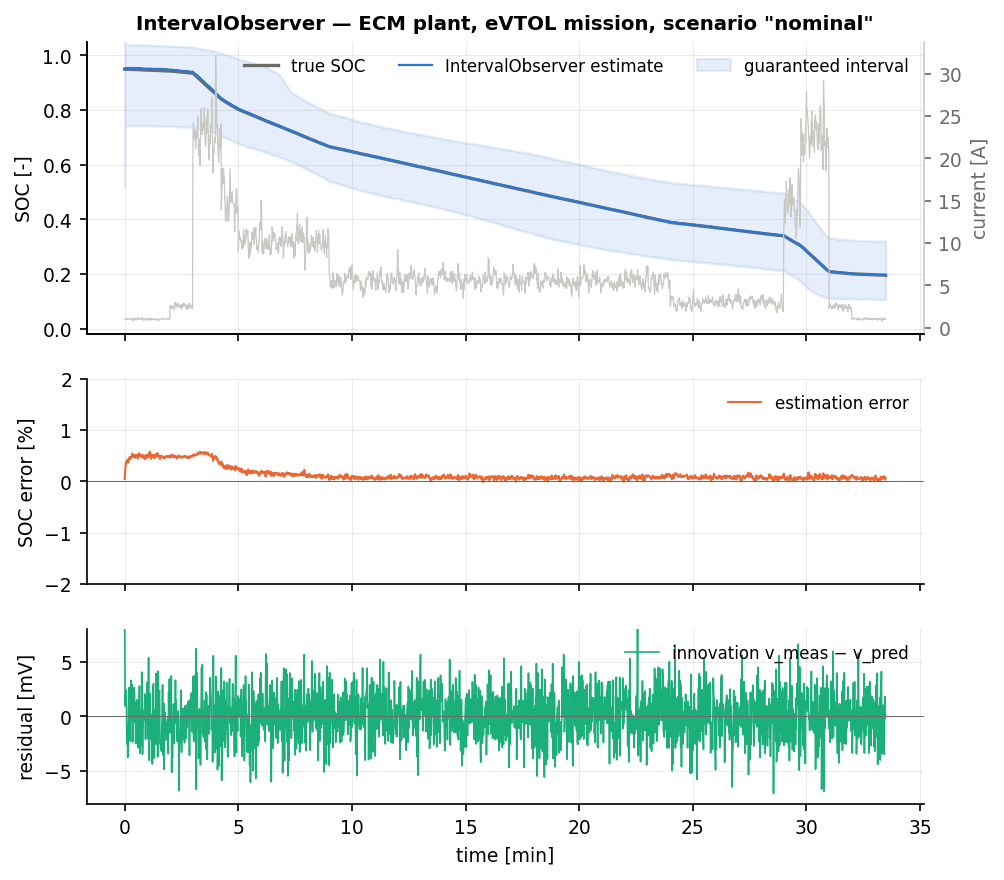
\includegraphics[width=\textwidth]{figures/cell_IntervalObserver_nominal.png}
\caption{IntervalObserver on the nominal eVTOL mission: true and estimated SOC (top), estimation error with the $\pm 2\sigma$ band when available (middle), voltage residual (bottom).}
\end{figure}
\begin{figure}[H]\centering
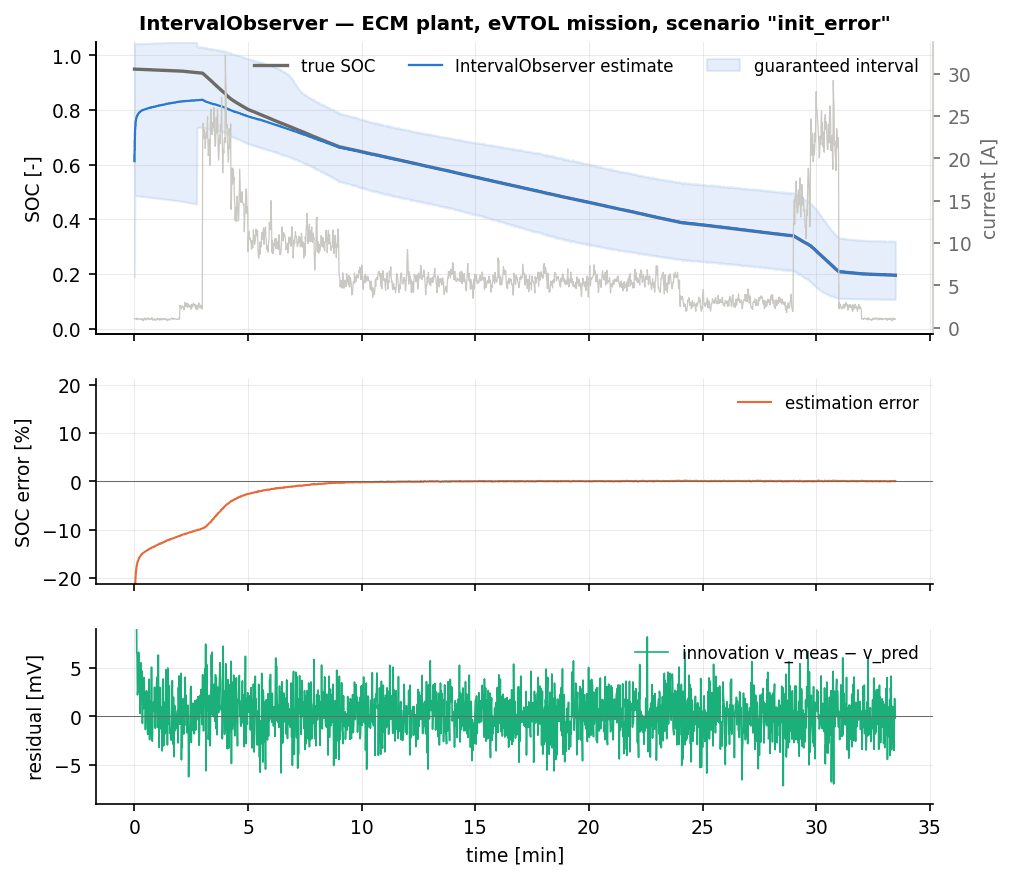
\includegraphics[width=\textwidth]{figures/cell_IntervalObserver_init_error.png}
\caption{IntervalObserver with a 35\,\% initial SOC error.}
\end{figure}

The headline metric is \texttt{bound\_violation}, the fraction of samples at which the true SOC
lies outside $[\soc_{\mathrm{lo}},\soc_{\mathrm{hi}}]$.  It is \textbf{exactly zero in all twelve
scenarios}, including \texttt{outliers} ($5\,\%$ of samples corrupted by $\pm50$\,mV),
\texttt{sensor\_dropout} (15\,s of stuck voltage), \texttt{param\_mismatch} ($-30\,\%$ on $R_0$),
\texttt{aged\_cell} ($-15\,\%$ capacity), \texttt{preisach} (structurally wrong hysteresis) and
\texttt{combined} (four simultaneous faults).  That is the property the method exists to provide,
and it is the only estimator in this study that provides it.

The price is the width: $0.274$ SOC on \texttt{nominal}, $0.252$ on \texttt{hot}, $0.368$ on
\texttt{cold} and $0.318$ on \texttt{combined}.  Decomposing \eqref{eq:io-width} for the nominal
case: $2\bar{v}/C_{\soc} = 2\times0.098/0.94 = 0.209$ from the measurement budget,
$\approx0.04$ from the RC widths, $\approx0.02$ from the SOC padding.  The measurement budget
dominates, and within it the $\pm50$\,mV outlier allowance dominates: a budget that excluded
outliers would give a width near $0.05$ but would then be violated in the \texttt{outliers}
scenario.  The \texttt{cold} case is wider because the RC time constants stretch by a factor of
three, so the open-loop growth of $w_{v_2}$ before the correction acts is larger.

As a point estimator the observer is now exactly as accurate as the \texttt{SSKF} it embeds
(\Cref{sec:io-point}): $\mathrm{rmse}_{ss} = 0.0008$ on \texttt{nominal}, $0.0031$ on
\texttt{cold}, $0.0203$ on \texttt{combined}, $0.0061$ and $0.0335$ on the single-particle plant's
\texttt{nominal} and \texttt{cold}, with the projection \eqref{eq:io-point} almost never binding.
The comparison with the midpoint is the point of the exercise: the midpoint gives $0.0110$,
$0.0196$, $0.0242$, $0.0238$ and $0.0600$ on the same five columns, between $1.2$ and $14$ times
worse, and on the SPM \texttt{nominal} column it is the only number in this family that fails the
$2\,\%$ acceptance threshold.  The bounds are unchanged by the substitution --- the violation count
is still zero and the mean widths are identical to three digits --- so this is a free improvement
of the reported estimate, not a loosening of the guarantee.

The \texttt{init\_error} column converges in $334$\,s with zero violations.

\section{Summary}
Use an interval observer when the deliverable is a guarantee rather than an estimate --- reserve
energy, a certification margin, a fault-detection threshold.  On this benchmark it encloses the
true SOC at every one of $240\,000$ samples across twelve fault scenarios, which no
covariance-based method can claim, at a run-time cost below the EKF's.  Exploit the cooperativity
of the plant, correct a single state, and neutralise the columns of $\mC$ whose sign blocks
monotonicity by widening with their known interval.  Budget the uncertainties honestly and expect
the width to be dominated by the measurement bound through $2\bar{v}/(\partial\ocv/\partial\soc)$;
narrowing that bound, not tuning the gain, is the way to a tighter interval.  Do not use the
midpoint as a point estimate when accuracy matters --- run a Luenberger or unknown-input observer
alongside it --- or, as here, embed one and project its output onto the interval, which costs
nothing and keeps the two answers consistent with each other.
